\subsection{IU3 Consultar Citas del paciente}

\subsubsection{Objetivo}
Mostrar al paciente la información de las citas que ha agendado en la clínica.

\subsubsection{Diseño}
Esta pantalla aparece al presionar el botón ``Consultar mis citas'' en la pantalla de inicio del Paciente.

\begin{figure}[htbp!]
	\centering
	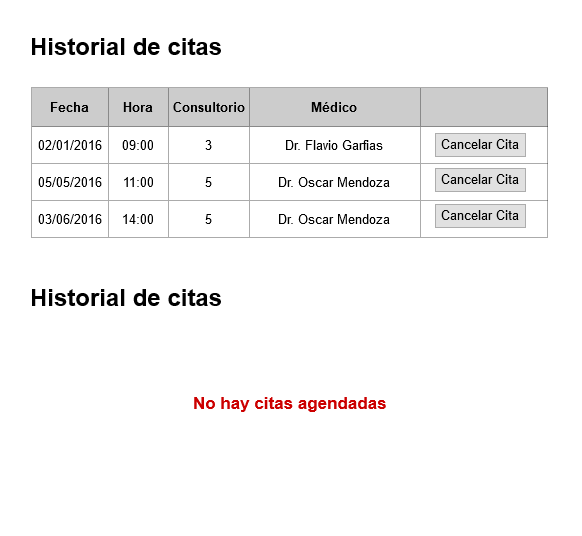
\includegraphics[width=0.8\textwidth]{images/gui/ui3_consultar_citas_paciente}
	\caption{Pantalla UI3 Consultar citas paciente}
\end{figure}

\subsubsection{Salidas}
\begin{itemize}
	\item Lista de citas.
\end{itemize}

\subsubsection{Entradas}
\begin{itemize}
	\item Ninguna. 
\end{itemize}

\subsubsection{Comandos}
\begin{itemize}
	\item \IUbutton{Cancelar cita}: Inicia CUX Cancelar cita.
\end{itemize}

\subsubsection{Mensajes}
\begin{Citemize}
	\item {\bf MSG3a} ``No hay citas agendadas''.
\end{Citemize}

\subsection{IU21 Consultar Pacientes}

\subsubsection{Objetivo}
Mostrar al gerente la información básica de los pacientes registrados en el sistema.

\subsubsection{Diseño}
Esta pantalla aparece al presionar el botón "Consultar Pacientes" en la pantalla de inicio del Gerente.

\begin{figure}[htbp!]
	\centering
	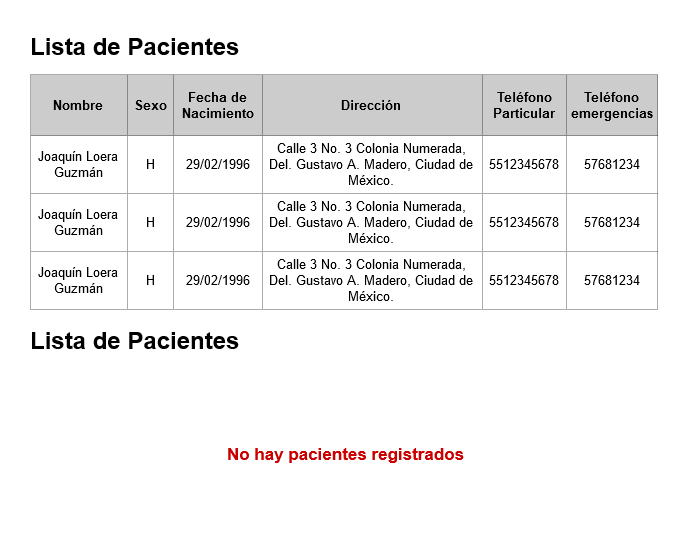
\includegraphics[width=0.8\textwidth]{images/gui/ui21_consultar_pacientes}
	\caption{Pantalla UI21 Consultar pacientes}
\end{figure}

\subsubsection{Salidas}
\begin{itemize}
	\item Lista de pacientes.
\end{itemize}

\subsubsection{Entradas}
\begin{itemize}
	\item Ninguna.
\end{itemize}

\subsubsection{Comandos}
\begin{itemize}
	\item Ninguno.
\end{itemize}

\subsubsection{Mensajes}
\begin{Citemize}
	\item {\bf MSG21a} ``No hay pacientes registrados''.
\end{Citemize}
